\documentclass[14pt, a4paper]{extarticle}
\usepackage{indentfirst}
\usepackage{titulpage}
\usepackage{listings}
\usepackage{color}

\textwidth 16cm
\textheight 25cm
\oddsidemargin -2.5mm
\evensidemargin -3mm
\topmargin -20mm
\parindent 1.25cm
\bibliography{sources.bib}

\begin{document}
    
    \fefutitlepage{Б9121-09.03.03пикд}{Яцевич К.А.}{2}{Февраля\hspace{30pt}}{23}
    \defaultfont
    
    \vspace{1cm}
   
    \pagebreak
   
    \tableofcontents
   
    \pagebreak

    \section*{Глоссарий}
    \addcontentsline{toc}{section}{Глоссарий}

    \textbf{Вершина(узел)} --- структурная единица графа

    \textbf{Ребро} --- соединяет вершины графа
    
    \textbf{Граф} --- математическая система, объекты которой обладают парными связями

    \textbf{Паросочетание} --- набор несмежных ребер

    \textbf{Свободная вершина} --- вершина графа, не покрытая паросочетанием

    \textbf{Дополняющий(увеличивающий) путь} --- чередующаяся цепь, которая начинается и кончается голыми вершинами.

    \textbf{Цветок(соцветие/бутон)} --- нечетный цикл графа

    \textbf{Стебель} --- чередующаяся цепь чётной длины

    \textbf{База} --- вершина графа, которая пренадлежит стеблю и  является частю цикла

    \pagebreak
   
    \section*{Введение}
    \addcontentsline{toc}{section}{Введение}
   
    % \textit{Цель:} Научиться определять тип ДУ, пользоваться методом Эйлера, и с помощью программ компьютерной математики научиться решать представленные ниже задачи.\\
   
    % \subsection*{Постановка задачи}
    % Требуется разработать алгоритм  за ассимтотику $O(n^3)$. Провести тестирование с использованием ручных тестов и тестов с использованием генератора.
   
    \subsection*{Историческая справка}
    \addcontentsline{toc}{subsection}{Историческая справка}
   
    Алгоритм разработал Джек Эдмондс в 1961 году и опубликовал в 1965 году. 
    
    Основной причиной, почему алгоритм сжатия цветков важен, является то, что он дал первое доказательство возможности нахождения наибольшего паросочетания за полиномиальное время. Другой причиной является то, что метод приводит к описанию многогранника линейного программирования для многогранника паросочетаний, что приводит к алгоритму паросочетания минимального веса. 
    
    Как уточнил Александр Схрейвер, дальнейшая важность результата следует из факта, что этот многогранник был первым, доказательство целочисленности которого «не просто следовало из тотальной унимодулярности, а его описание было прорывом в комбинаторике многогранников».

    \pagebreak
    
    \section*{Описание алгоритма}
    \addcontentsline{toc}{section}{Описание алгоритма}

    \subsection*{Идея алгоритма}
    \addcontentsline{toc}{subsection}{Идея алгоритма}
    
    Алгоритм сжатия цветков (англ. Blossom algorithm) — это алгоритм в теории графов для построения наибольших паросочетаний на графах.
    
    Если дан граф $G=(V, E)$ общего вида, алгоритм находит паросочетание M такое, что каждая вершина из $V$ инцидентна не более чем одному ребру из $M$ и $|M|$ максимально. Паросочетание строится путем итеративного улучшения начального пустого паросочетания вдоль увеличивающих путей графа. 
    
    В отличие от двудольного паросочетания ключевой новой идеей было сжатие нечетного цикла в графе (цветка) в одну вершину с продолжением поиска итеративно по сжатому графу.

    \subsection*{Оценка сложности}
    \addcontentsline{toc}{subsection}{Оценка сложности}

    Всего имеется $n$ итераций, на каждой из которых выполняется обход в ширину за $O(m)$ кроме того, могут происходить операции сжатия цветков — их может быть $O(n_1)$. Сжатие соцветий работает за $O(n_2)$, стоит отметить $n_1 \equiv n_2$, то есть общая асимптотика алгоритма составит $O(n(m+n^2))=O(n^3)$.

    \subsection*{Нахождение дополняющего(увеличивающего) пути}
    \addcontentsline{toc}{subsection}{Нахождение дополняющего(увеличивающего) пути}

    Пусть зафиксировано некоторое паросочетание $M$. Тогда простая цепь $P = (v_1, v_2, \ldots, v_k)$ называется чередующейся цепью, если в ней рёбра по очереди принадлежат --- не принадлежат паросочетанию $M$. Чередующаяся цепь называется увеличивающей, если её первая и последняя вершины не принадлежат паросочетанию. Иными словами, простая цепь $P$ является увеличивающей тогда и только тогда, когда вершина $v_1 \not\in M$, ребро $(v_2,v_3) \in M$, ребро $(v_4,v_5) \in M$, ..., ребро $(v_{k-2},v_{k-1}) \in M$, и вершина $v_k \not\in M$.

    Мы сможем найти максимальное паросочитание путем инверсии дополняющего пути.

    Основная проблема заключается в том, как находить увеличивающий путь. Если в графе имеются циклы нечётной длины, то просто обход в глубину/ширину будет работать не корректно --- при попадании в цикл нечётной длины обход может пойти по циклу в неправильном направлении.

    \pagebreak

    \subsection*{Сжатие цветка}
    \addcontentsline{toc}{subsection}{Сжатие цветка}

    \textbf{Сжатие цветка} — это сжатие всего нечётного цикла в одну псевдо-вершину (соответственно, все рёбра, инцидентные вершинам этого цикла, становятся инцидентными псевдо-вершине).
    
    \subsection*{Теорема Эдмондса}
    \addcontentsline{toc}{subsection}{Теорема Эдмондса}

    Пусть граф $\overline G$ был получен из графа G сжатием одного цветка.
    Тогда в графе $\overline G$ существует увеличивающая цепь тогда и только тогда, когда существует увеличивающая цепь в $G$.

    \textit{Доказательство}. 
    
    Обозначим через B цикл цветка, и через $\overline B$ соответствующую сжатую вершину.
    Вначале заметим, что достаточно рассматривать случай, когда база цветка является свободной вершиной (не принадлежащей паросочетанию). Действительно, в противном случае в базе цветка оканчивается чередующийся путь чётной длины, начинающийся в свободной вершине. Прочередовав паросочетание вдоль этого пути, мощность паросочетания не изменится, а база цветка станет свободной вершиной. Итак, при доказательстве можно считать, что база цветка является свободной вершиной.

    Пусть путь $P$ является увеличивающим в графе $G$. Если он не проходит через B, то тогда, очевидно, он будет увеличивающим и в графе $\overline G$. Пусть P проходит через B. Тогда можно считать, что путь P представляет собой некоторый путь $P_1$, не проходящий по вершинам B, плюс некоторый путь $P_2$, проходящий по вершинам B и, возможно, другим вершинам. Но тогда путь $P_1$ + $\overline B$ будет являться увеличивающим путём в графе $\overline G$, что и требовалось доказать.

    \pagebreak
    
    \subsection*{Общая схема алгоритма}
    \addcontentsline{toc}{subsection}{Общая схема алгоритма}

    \begin{figure}[h!]
        \centering
        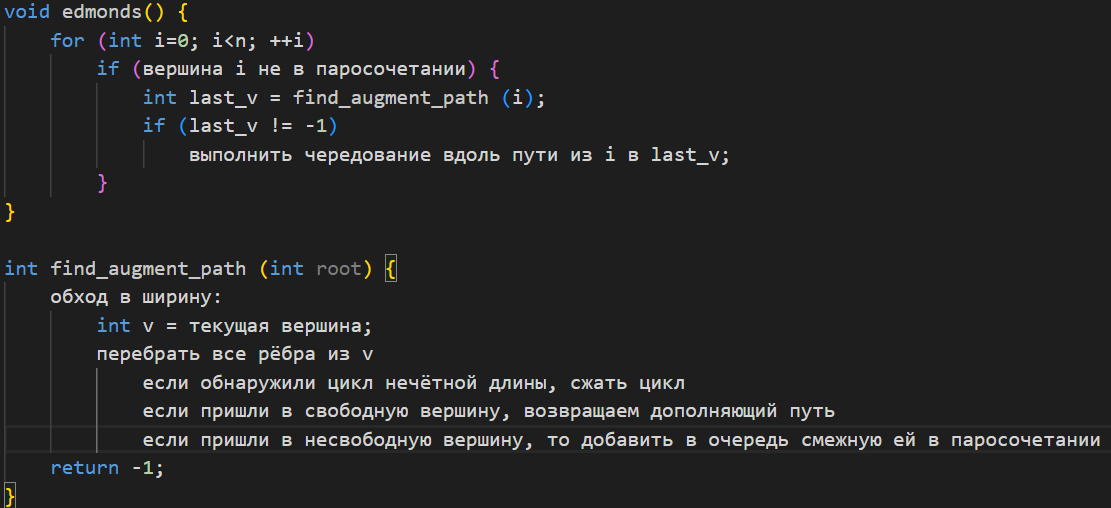
\includegraphics[scale=0.9]{psevdo.png}
        \label{fig:my_label}
    \end{figure}

    \pagebreak
    
    \subsection*{Пример работы алгоритма}
    \addcontentsline{toc}{subsection}{Пример работы алгоритма}


    \begin{figure}[h!]
        \centering
        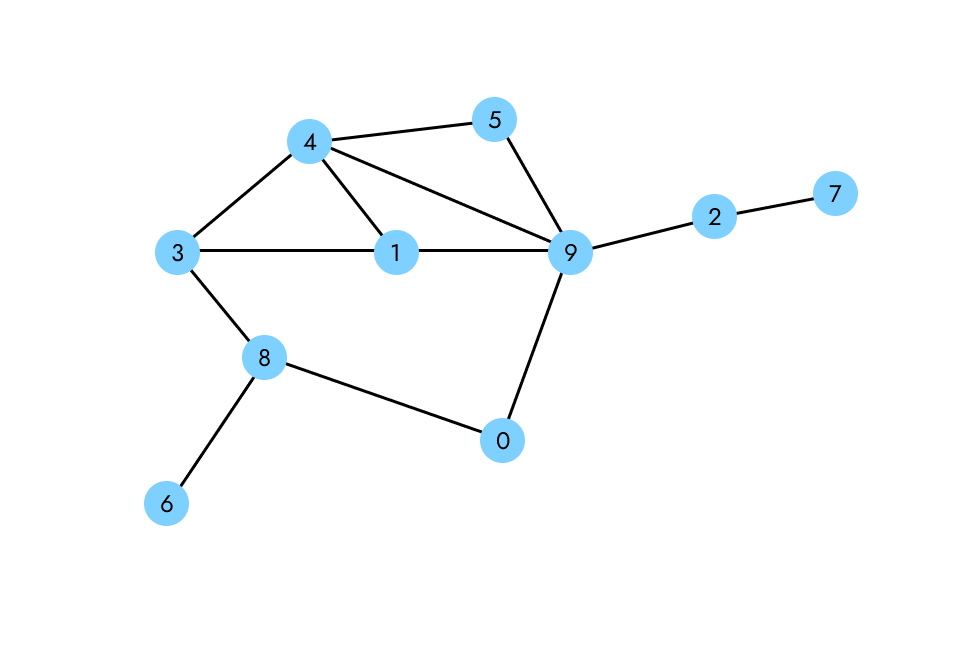
\includegraphics[scale=0.3]{1.png}
        \caption{Исходный граф}
        \label{fig:my_label}
    \end{figure}

    Начинаем рассматривать граф со свободной вершины 7. Двигаясь по ребрам обнаруживаем стебель: ребра 7-2 и  2-9. Следовательно, предполагаемый дополняющий путь будет начинаться со свободной вершины 7, ребро 2-9 --- паросочетание. Тогда вершина 9 является базой. С помощию BFS идем дальшне по графу:
    ребро 9-5, ребро 5-4, ребро 4-9 --- составляют нечетный цикл --- цветок.
    
    \begin{figure}[h!]
        \centering
        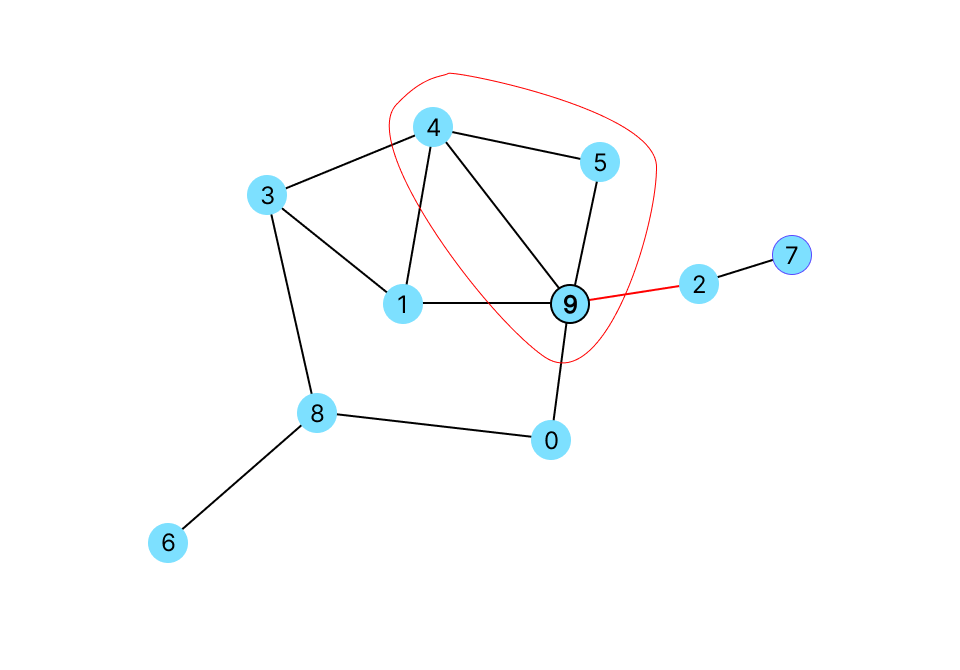
\includegraphics[scale=0.3]{2.png}
        \caption{Нахождение первого цветка}
        \label{fig:my_label}
    \end{figure}

    
    Вершины цикла сжимаем в базу. Получаем следующий граф, который продолжаем обрабатывать по тому же алгоритму.
    С помощию BFS идем дальше по графу:
    ребро 9-3, ребро 3-1, ребро 1-9 --- составляют нечетный цикл --- цветок.

    \begin{figure}[h!]
        \centering
        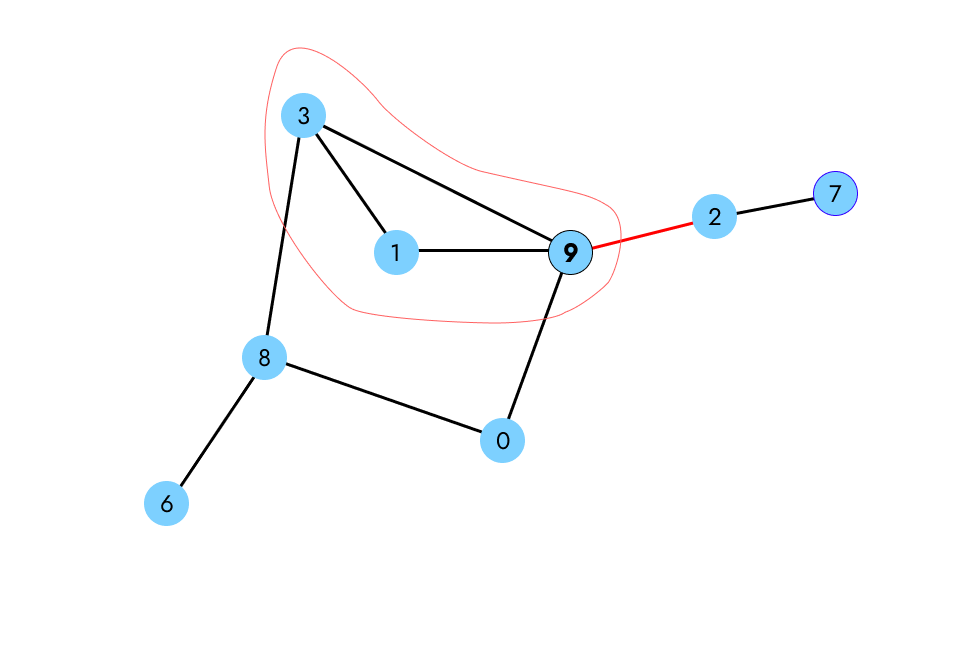
\includegraphics[scale=0.3]{3.png}
        \caption{Нахождение второго цветка}
        \label{fig:my_label}
    \end{figure} 

    \pagebreak

    Вершины цикла сжимаем в базу. Новый  граф снова обрабатываем.
    Ребра 9-8 8-0 и 0-9 --- составляют нечетный цикл --- цветок.

    \begin{figure}[h!]
        \centering
        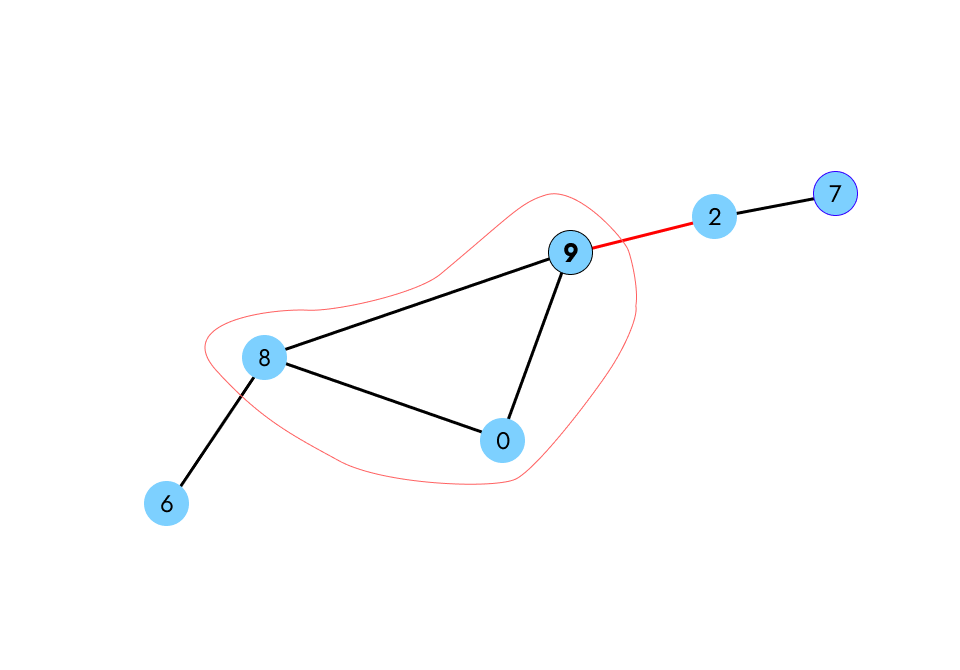
\includegraphics[scale=0.3]{4.png}
        \caption{Нахождение третьего цветка}
        \label{fig:my_label}
    \end{figure} 

    Сжимаем цветок и продолжаем анализировать граф. После базы 9 идет только одно ребро 9-6, окончание которого --- свободная вершина 6. Следовательно можем утверждать, что мы нашли дополняющий путь: 7-2, 2-9, 9-6.

    \begin{figure}[h!]
        \centering
        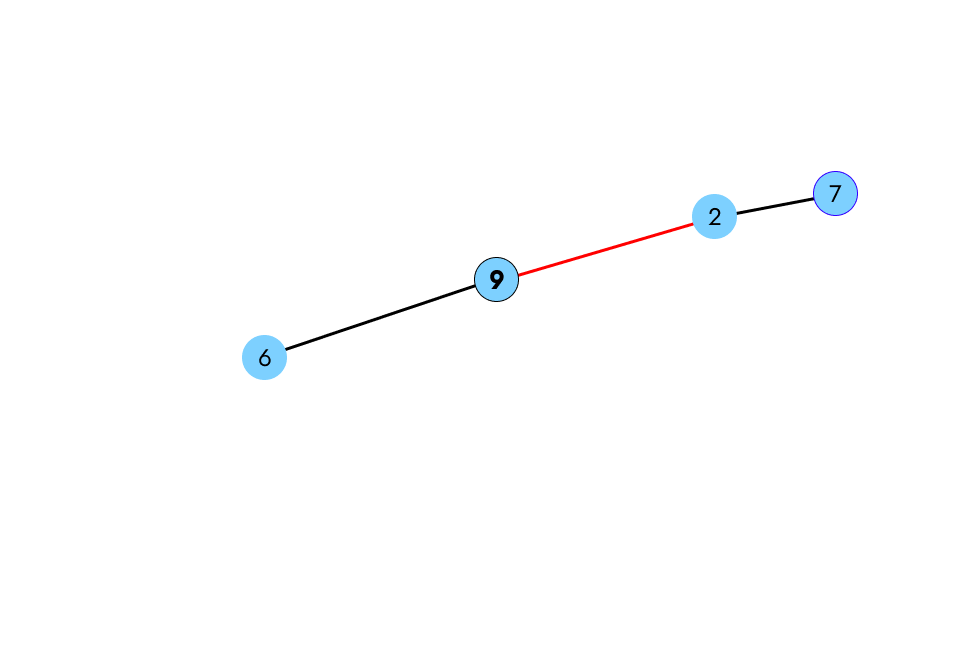
\includegraphics[scale=0.3]{5.png}
        \caption{Дополняющий путь}
        \label{fig:my_label}
    \end{figure} 

    \pagebreak

    Обращаемся к теореме Эдмондса:
    
    В графе $\overline G$ существует увеличивающая цепь тогда и только тогда, когда существует увеличивающая цепь в $G$.

    Значит мы можем приступить к восстановлению графа путем последовательного возвращения цветков.
    Для нахождения максимального паросочетания начнём с инверсии дополняющего пути.
    Начинаем восстановление с последнего сжатия цветка, инвертируя путь. При этом инвертрование пути подразумевает переопределение паросочетания. В цветке мы определяем паросочетание "в обратной последовательности": начиная с 9-0, переходя к 0-8. Так как в дополняющем пути база 9 была соединена с вершиной 6, то дойдя до узла, соединенного с вершиной 6, мы продолжаем переопределять паросочетание в направлении вершины 6.

    На данном этапе паросочетание составляет следующие не инцидентные ребра:
    7-2, 9-0, 8-6

    \pagebreak
    
    \begin{figure}[h!]
        \centering
        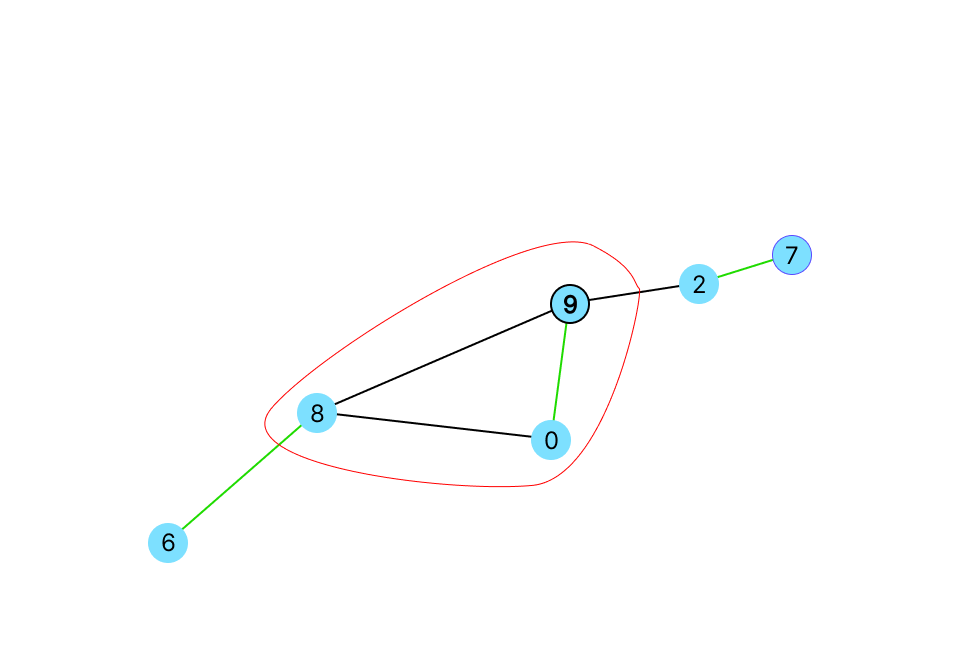
\includegraphics[scale=0.3]{6.png}
        \caption{Восстановление третьего цветка}
        \label{fig:my_label}
    \end{figure} 

    Запоминаем проставленное паросочетание и продолжаем восстановление графа. Ребро 7-2 уже инвертированно, поэтому переходим сразу к базе: в цветке определяем паросочетание "в обратной последовательности". База уже относится к ребру паросочетания, поэтому мы не можем пометить ребро 9-1. Значит помечаем следующее ребро 1-3. Аналогично с ребром 3-9.  

    На данном этапе паросочетание составляет следующие не инцидентные ребра:
    7-2, 9-0, 8-6, 3-1
    
    \begin{figure}[h!]
        \centering
        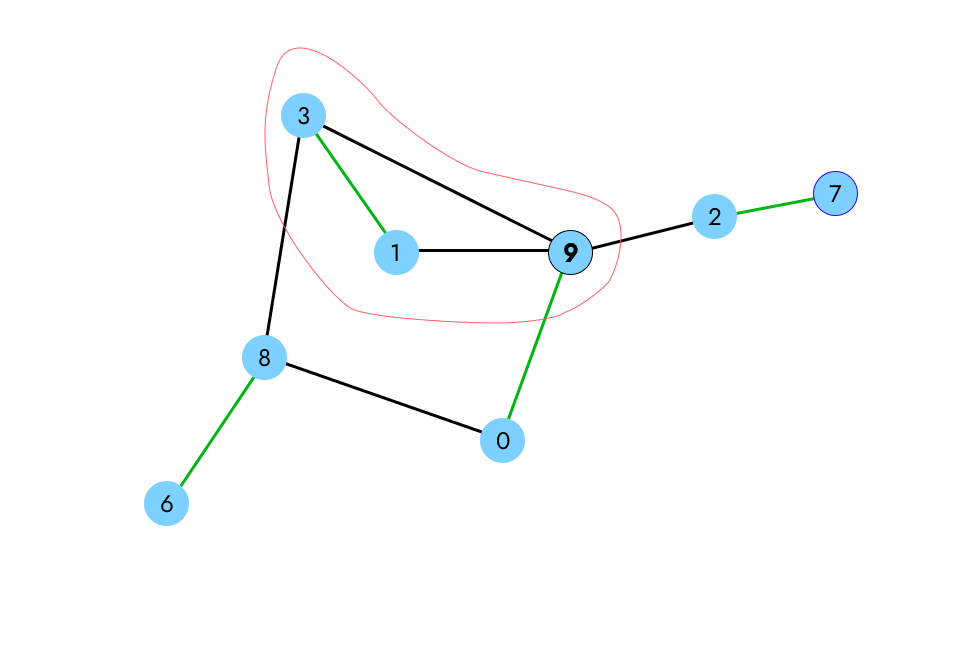
\includegraphics[scale=0.3]{7.png}
        \caption{Восстановление второго цветка}
        \label{fig:my_label}
    \end{figure} 

    \pagebreak

    Восстанавливаем последний цветок: аналогично помечаем ребра, начиная с базы. Ребро 9-4 --- не помечаем, ребро 4-5 --- помечаем, ребро 5-9 --- не помечаем. 

    \begin{figure}[ht!]
        \centering
        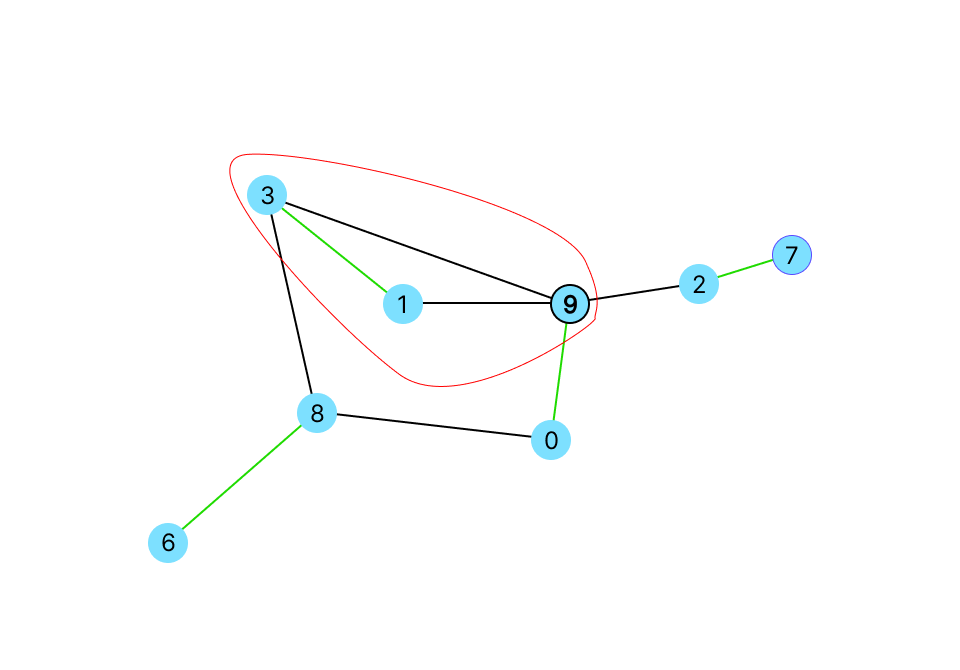
\includegraphics[scale=0.3]{8.png}
        \caption{Восстановление первого цветка}
        \label{fig:my_label}
    \end{figure} 

    Мы закончили восстановление графа и нашли максимальное паросочетание.

    \pagebreak
    
    \section*{Реализация}
    \addcontentsline{toc}{section}{Реализация}

    %\subsection*{Представление графа}
    %\addcontentsline{toc}{subsection}{Представление графа}
    
    \subsection*{Нахождение ближайшего предка}
    \addcontentsline{toc}{subsection}{Нахождение ближайшего предка}

    \begin{lstlisting}[language=c++]
int lca(int a, int b) {
	bool used[MAXN] = { 0 };
 
	for (;;) {
		a = base[a];
		used[a] = true;
		if (match[a] == -1)  break; // дошли до корня
		a = p[match[a]];
	}
 
	for (;;) {
		b = base[b];
		if (used[b])  return b;
		b = p[match[b]];
	}
}
    \end{lstlisting}


    \subsection*{Обозначение дополняющего пути}
    \addcontentsline{toc}{subsection}{Обозначение дополняющего пути}
    \begin{lstlisting}[language=c++]
void mark_path(int v, int b, int children) {
    while (base[v] != b) {
        blossom[base[v]] = blossom[base[match[v]]] = true;
        p[v] = children;
        children = match[v];
        v = p[match[v]];
    }
} 
    \end{lstlisting}

    \pagebreak

    \subsection*{Поиск дополняющего пути}
    \addcontentsline{toc}{subsection}{Поиск дополняющего пути}

    \begin{lstlisting}[language=c++]
int find_path(int root) {
    memset(used, 0, sizeof used);
    memset(p, -1, sizeof p);
    for (int i = 0; i < MAXN; i++)
        base[i] = i;
    
    used[root] = true;
    int qh = 0, qt = 0;
    q[qt++] = root;
    while (qh < qt) {
        int v = q[qh++];
        for (size_t i = 0; i < g[v].size(); i++) {
            int to = g[v][i];
            if (base[v] == base[to] || match[v] == to)  
                continue;
            if (to == root || match[to] != -1 && p[match[to]] != -1) {
                int curbase = lca(v, to);
                memset(blossom, 0, sizeof blossom);
                mark_path(v, curbase, to);
                mark_path(to, curbase, v);
                for (int i = 0; i < MAXN; i++)
                    if (blossom[base[i]]) {
                        base[i] = curbase;
                        if (!used[i]) {
                            used[i] = true;
                            q[qt++] = i;
                        }
                    }
            }
            else if (p[to] == -1) {
                p[to] = v;
                if (match[to] == -1)
                    return to;
                to = match[to];
                used[to] = true;
                q[qt++] = to;
            }
        }
    }
    return -1;
    \end{lstlisting}


    %\section*{Оптимизация}
    %\addcontentsline{toc}{section}{Оптимизация}

    %\subsection*{Возможная оптимизация}
    %\addcontentsline{toc}{subsection}{Возможная оптимизация}
    
    %\section*{Тестирование}
    %\addcontentsline{toc}{section}{Тестирование}

    \pagebreak

    \begin{thebibliography}{}
    
    \bibitem{1} 
    ИТМО, Викиконспекты --- Алгоритм вырезания соцветий.  4 сентября 2022. 

    \bibitem{2} 
    MAXimal --- Алгоритм Эдмондса нахождения наибольшего паросочетания в произвольных графах. 6 декабря 2012.\\
    
    \bibitem{3}
    Энциклопедии Руниверсалис --- Алгоритм сжатия цветков.  28 ноября 2022.\\
    
    \bibitem{4}
    Единый центр по исследованию искусственного интеллекта "ЕЦИИИ" --- Алгоритм вырезания соцветий и сжатия цветков.\\
    
    \end{thebibliography}    
    
    \addcontentsline{toc}{section}{Список литературы}
    \printbibliography
    
\end{document}